%general
\title{\LARGE\textsc{Thermalization of Gluons \\in\\ Relativistic Collisions}}
\author{\textbf{\large Mathieu Kaltschmidt} \\ITP Heidelberg}
\date{Statistical Physics Seminar \\
supervised by \\ Prof. Georg Wolschin \\[1em]
Heidelberg, July 3rd 2020}

%\titlegraphic{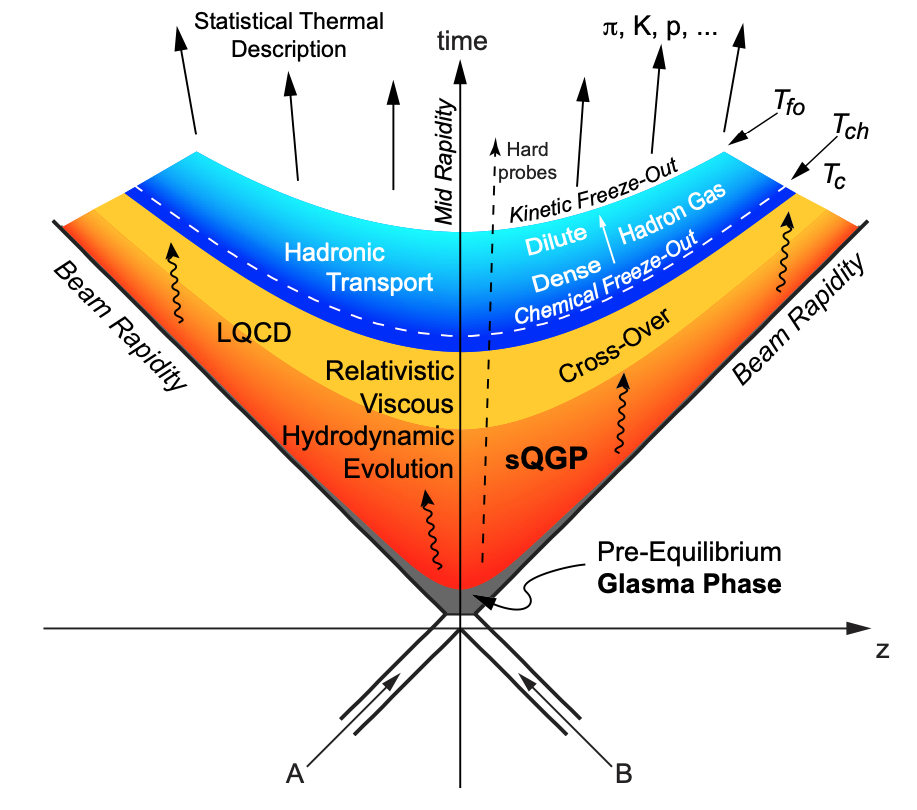
\includegraphics[width=6cm]{figures/rhic_schematic}}



%beamer style and individual color settings
\useinnertheme{circles}
\beamertemplatenavigationsymbolsempty
\setbeamersize{text margin left = 1.5em}
\setbeamersize{text margin right = 1.5em}

\setbeamercolor{frametitle}{fg=HDRed}
\setbeamercolor{part title}{fg=HDRed}
\setbeamercolor{title}{fg=HDRed}
\setbeamercolor{math text}{fg=DarkBlue}
\setbeamercolor{alerted text}{fg=HDRed}

\setbeamercolor{item}{fg=HDRed}
\setbeamercolor{bibliography item}{fg=DarkBlue}
\setbeamercolor{bibliography entry author}{fg=DarkBlue}

%fonts
\usepackage{fontspec}
%\usefonttheme{structurebold}
%\setsansfont{Palatino}
\usefonttheme[onlymath]{serif}


%page numbering
\setbeamertemplate{footline}[page number]
\setbeamercolor{page number in head/foot}{fg=black}
\setbeamerfont{page number in head/foot}{size=\small}

%math and theorems
\usepackage{amsmath}
\usepackage{amssymb}

%language settings 
\usepackage{polyglossia}
\setmainlanguage{english}


%useful packages
\usepackage{appendixnumberbeamer}
\usepackage{booktabs}
\usepackage{siunitx}
\usepackage{graphicx}
\usepackage{float}
\usepackage{blindtext}
\usepackage{physics}
\usepackage[labelfont=bf]{caption}

%Color Settings
\usepackage{xcolor}
\definecolor{HDRed}{RGB}{157,0,0}
\definecolor{DarkBlue}{RGB}{1,1,141}
\definecolor{DarkGreen}{RGB}{0, 119, 85}

% nice fracs
\usepackage{xfrac}

%bib settings
\usepackage[
	bibstyle=numeric-comp,
	%citestyle=authoryear,
	backend=biber,
	isbn=false,
	date=year,
	url=false,
	doi=false,
	hyperref = auto, 
	maxnames=99,
	backref, 
	backrefstyle=none]{biblatex}
\addbibresource{bibliography/statphyssem.bib}

%citation style
\renewcommand*{\citesetup}{%
  \footnotesize
  \color{DarkGreen}
  \biburlsetup
  \frenchspacing}
 
%numbering in bib
\setbeamertemplate{bibliography item}[text]

%linebreaks between author and title etc.
\DeclareDelimFormat[bib]{nametitledelim}{\newline\bibsentence}
\usepackage{xpatch}
\makeatletter
\def\do#1{
  \ifcsdef{blx@bbx@#1}
    {\xpatchbibdriver{#1}
       {\printlist{language}%
        \newunit\newblock}
       {\printlist{language}%
        \printunit{\newline\bibsentence}}
       {}{}}
    {}} 
\abx@doentrytypes
\makeatother

%suppress "In:" and quotation marks
\renewbibmacro{in:}{}
\DeclareFieldFormat[article,inbook,incollection,inproceedings,patent,thesis,unpublished]
  {title}{#1\isdot}
  
%own citation style
\newcommand{\mycite}[1]{\\\hfill\footnotesize\color{DarkGreen}\citeauthor{#1} (\citeyear{#1})\normalsize\normalcolor}

%tikz
\usepackage{tikz}
\usetikzlibrary{shapes, patterns, hobby}
\usepackage{pgfplots}
\usepgfplotslibrary{fillbetween}
\usetikzlibrary{positioning,arrows}

%highlighted toc at beginning of every section
\AtBeginSection[]
{
\begin{frame}[plain]
  \frametitle{Outline}
  \tableofcontents[currentsection]
\end{frame}
}

